% {{{ Paquetes, comandos etc
%%
%%	AVISO IMPORTANTE
%%	Formato optimizado para el sistema operativo GNU/Linux 64 bits
%%	usar TexLive 2016 (o superior), http://www.ctan.org/tex-archive/systems/texlive/Images/
%%	usar TeXstudio 2.11, http://texstudio.sourceforge.net/

\documentclass[letterpaper,12pt]{thesisECFM}
\usepackage{macros}

%%	NO OLVIDE INCLUIR FUENTE DE LAS TABLAS Y FIGURAS

% Descomentar para anular recuadros en los hiperenlaces dentro del pdf
\hypersetup{pdfborder={0 0 0}}

% Teoremas ---------------------------------------------------------
% estos ambientes son para teoremas, lemas, corolarios, otros
% si no los utiliza los puede obviar en su trabajo de graduación
\theoremstyle{plain}
\newtheorem{thm}{Teorema}[section]
\newtheorem{cor}{Corolario}[chapter]
\newtheorem{lem}{Lema}[chapter]
\newtheorem{prp}{Proposición}[chapter]

\theoremstyle{definition}
\newtheorem{exa}{Ejemplo}[chapter]
\newtheorem{defn}{Definición}[chapter]
\newtheorem{axm}{Axioma}[chapter]
\usepackage[draft,inline,nomargin]{fixme} \fxsetup{theme=color}
\FXRegisterAuthor{cp}{acp}{\color{blue}CP}
\FXRegisterAuthor{fel}{afel}{\color{red}F}

\theoremstyle{remark}
\newtheorem{rem}{Nota}[chapter]

% <<<<<<<<<<<<<<<<<<<<<<<<<<<<<<<<<<<<<>>>>>>>>>>>>>>>>>>>>>>>>>>>>>>>>>>>>>>>>
% <<<<<<<<<<<<<<                                             >>>>>>>>>>>>>>>>>>
%                 Inicio preámbulo de José Alfredo de León
% <<<<<<<<<<<<<<                                             >>>>>>>>>>>>>>>>>>
% <<<<<<<<<<<<<<<<<<<<<<<<<<<<<<<<<<<<<>>>>>>>>>>>>>>>>>>>>>>>>>>>>>>>>>>>>>>>>



%\usepackage{lscape}		%% para poner tablas en orientación landscape
\usepackage{array}		%% para modificar cosas de entorno 'tabular'
\newcolumntype{P}[1]{>{\centering\arraybackslash}m{#1}} %para que en las tablas quede centrado verticalmente el texto


%% símbolos de mate y física --------------------------------------------------
\usepackage{amssymb}	
\usepackage{amsbsy}
\usepackage{physics}
%% ----------------------------------------------------------------------------


\usepackage{longtable}	%% tablas en más de una página
\usepackage{float}		%% para poder usar H, h! en entornos table y figure, por ej.

%% para poner subfiguras
\usepackage{caption} 
\usepackage{subcaption}

\usepackage{lipsum} % para poner texto equis
\usepackage{rotating} % para poner tablas rotadas

%%% ----------------------------------------------------------------------------
%% \usepackage[inline]{showlabels}		%% para mostrar labels en el PDF
		
			
\usepackage{graphicx}			%% para colocar imágenes
\graphicspath{ {./img/} }		%% ruta a carpeta con imágenes


%% Para enumerar las líneas del PDF -------------------------------------------
%\usepackage[]{lineno} %\linenumbers
%\setlength\linenumbersep{3pt}
%% para que funcione mejor la numeración {{{
%% https://tex.stackexchange.com/questions/43648/why-doesnt-lineno-number-a-paragraph-when-it-is-followed-by-an-align-equation
%\newcommand*\patchAmsMathEnvironmentForLineno[1]{%
%  \expandafter\let\csname old#1\expandafter\endcsname\csname #1\endcsname
%  \expandafter\let\csname oldend#1\expandafter\endcsname\csname end#1\endcsname
%  \renewenvironment{#1}%
%     {\linenomath\csname old#1\endcsname}%
%     {\csname oldend#1\endcsname\endlinenomath}}% 
%\newcommand*\patchBothAmsMathEnvironmentsForLineno[1]{%
%  \patchAmsMathEnvironmentForLineno{#1}%
%  \patchAmsMathEnvironmentForLineno{#1*}}%
%\AtBeginDocument{%
%\patchBothAmsMathEnvironmentsForLineno{equation}%
%\patchBothAmsMathEnvironmentsForLineno{align}%
%\patchBothAmsMathEnvironmentsForLineno{flalign}%
%\patchBothAmsMathEnvironmentsForLineno{alignat}%
%\patchBothAmsMathEnvironmentsForLineno{gather}%
%\patchBothAmsMathEnvironmentsForLineno{multline}%
%}
%% }}}	
%% ----------------------------------------------------------------------------


%%%%%%%%%%%%   Inicio definición de comandos   %%%%%%%%%%%%%%%%
\newcommand{\fref}[1]{fig.~\ref{#1}}   \newcommand{\tref}[1]{tabla~\ref{#1}}     
\newcommand{\Fref}[1]{Fig.~\ref{#1}}  \newcommand{\Tref}[1]{Tabla~\ref{#1}}
\newcommand{\Cref}[1]{Cuadro~\ref{#1}}
\newcommand{\psii}{\psi_i}
\newcommand{\Pk}[1]{\ket{\psi_{#1} }}
\newcommand{\Pb}[1]{\bra{\psi_{#1} }}
\newcommand{\pk}{\ket{\psi}}
\newcommand{\M}{\mathcal{M}^{(N)}}
\newcommand{\E}{\mathcal{E}}
\newcommand{\Erho}{\mathcal{E}(\rho)}
\newcommand{\1}{\mathbb{1}}
\newcommand{\ten}{\otimes}
\newcommand{\h}[1]{\colorbox{yellow}{#1}}
\newcommand{\hi}{\mathcal{H}}
\newcommand{\txt}[1]{\text{#1}}
\newcommand{\here}{\h{\hspace{15cm}} }
\newcommand{\rhoi}{\dyad{\psii}{\psii}}
\newcommand{\ind}[2]{{{}^{#1}_{#2}}}
\newcommand{\rc}[1]{r_{#1}}
\newcommand{\pauli}[2]{\sigma_{#1}\otimes\sigma_{#2}}
\newcommand{\esqueleto}[1]{\textcolor{JAsColor}
{\noindent\textbf{Esqueleto:} #1}}
\newcommand{\ot}{\otimes}
\newcommand{\m}{\textcolor{JAsColor}{|}}
\newcommand{\taus}{\tau_{j_1,\ldots ,j_n}}
\newcommand{\tauijk}[3]{\boldmath{$\tau_{#1#2#3}$}}
\newcommand{\tauij}[2]{\boldmath{$\tau_{#1#2}$}}
\newcommand{\ep}{\textbf{Fuente:} elaboración propia.}
\newcommand{\subind}[2]{{}_{#1}^{#2}}
\newcommand{\ruskaiMap}{canal diagonal de Pauli constante sobre los ejes}
\newcommand{\ruskai}{canales diagonales de Pauli constantes sobre los ejes}
%%%%%%%%%%%   Fin definición de comandos   %%%%%%%%%%%%%%%%%%


% Cosas que no sé porqué tengo ------------------------------------------------
\usepackage{natbib}
\usepackage{ctable} 
\usepackage{bbold}
\usepackage{fancybox}	
\usepackage{colortbl}

\renewcommand{\labelenumii}{\arabic{enumi}.\arabic{enumii}}
\renewcommand{\labelenumiii}{\arabic{enumi}.\arabic{enumii}.\arabic{enumiii}}
\renewcommand{\labelenumiv}{\arabic{enumi}.\arabic{enumii}.\arabic{enumiii}.\arabic{enumiv}}

\renewcommand{\thefootnote}{\fnsymbol{footnote}}


% <<<<<<<<<<<<<<<<<<<<<<<<<<<<<<<<<<<<<>>>>>>>>>>>>>>>>>>>>>>>>>>>>>>>>>>>>>>>>
% <<<<<<<<<<<<<<                                             >>>>>>>>>>>>>>>>>>
%                   Fin preámbulo de José Alfredo de León
% <<<<<<<<<<<<<<                                             >>>>>>>>>>>>>>>>>>
% <<<<<<<<<<<<<<<<<<<<<<<<<<<<<<<<<<<<<>>>>>>>>>>>>>>>>>>>>>>>>>>>>>>>>>>>>>>>>



% Cuerpo de la tesis -----------------------------------------------

% Preámbulo
% }}}
\begin{document}

% Datos generales del trabajo de graduación, tabla de contenidos etc {{{
\datosThesis%
{1}%						% física 1; matemática 2
{Implementación de canales cuánticos \\ de un qubit usando VQA}%		% Título del trabajo de graduación
{Felipe Antonio Ixcamparic Choy}%			% autor
{M.Sc. Juan Diego Chang\\y Dr. Carlos Francisco Pineda Zorrilla}%			% asesor
{agosto de 2024}		% mes y año de la orden de impresión
{2}							% femenino 1; masculino 2

\tableofcontents    % Índice general vinculado

% Inicio del contenido principal
\mainmatter
% }}}
\chapter*{OBJETIVOS} % {{{
\section*{General} 
\cpnote{Por favor consistencia con la capitalizacion de ``Algoritmos Variacionales''.}
Estudiar  y desarrollar algoritmos variacionales cuánticos para la implementación de canales cuánticos de un \textit{qubit} en computadoras cuánticas.

\section*{Específicos}
\begin{itemize}
    \item Estudiar la teoría y uso de computadoras cuánticas.
    \item Comprender las definiciones fundamentales de la teoría de sistemas cuánticos abiertos y canales cuánticos.
    \item Investigar el uso de los Algoritmos Variacionales Cuánticos en la resolución de problemas de información cuántica.
    \item Implementar canales cuánticos de un qubit en computadoras cuánticas y analizar su comportamiento.
\end{itemize}
% }}}
\chapter*{INTRODUCCIÓN} % {{{
El estudio de la dinámica de sistemas cuánticos abiertos es fundamental para el avance de la computación e información cuántica. Los canales cuánticos describen la evolución de estados cuánticos en  interacción con su entorno, y son clave para el entendimiento de este tipo de sistemas.

En este trabajo, nos enfocamos en la aplicación de Algoritmos Variacionales Cuánticos (VQA) para la inicialización y optimización de canales cuánticos en plataformas de computación cuántica. Los VQA, a través de su enfoque híbrido que combina computación cuántica y optimización clásica, nos ofrecen una técnica óptima para ajustar los parámetros que gobiernan los canales cuánticos, permitiendo una mayor precisión y control en el procesamiento cuántico.

% }}}
\chapter{FUNDAMENTOS TEÓRICOS} % {{{
\section{Introducción}

\section{Matriz Densidad}
*Sección heredada de informe de prácticas

Un sistema cuántico se describe mediante un vector complejo $\ket{\psi}$, conocido como estado cuántico. Un estado cuántico puro se representa como:
$
\ket{\psi} = \sum_{i=1}^{d} c_i \ket{i},
$
donde $c_i$ son coeficientes complejos y $\{\ket{i}\}$ es una base ortonormal. Los coeficientes deben cumplir con la condición de normalización:
$
\braket{\psi}{\psi}=1.
$ \par 
Los estados puros pueden representarse mediante la matriz densidad:$\rho = \ketbra{\psi}.$. \par   
 
Un estado mixto es un ensamble estadístico de estados puros $\{\ket{\psi_i}\}$ con probabilidades $\{p_i\}$. La matriz densidad para estados mixtos es:$\rho = \sum_{i=1}^{n} p_i \ketbra{\psi_i}.$ \par 

La matriz densidad $\rho$ tiene tres propiedades principales: Hermiticidad , traza unitaria y no negatividad. \par

La pureza de un estado cuántico mide qué tan mixto es el estado. Se define como $\text{Pureza} = tr(\rho^2).$ \par

La traza parcial se usa para obtener la matriz densidad reducida de un subsistema en estados compuestos. Por ejemplo, si tenemos un sistema compuesto por dos subsistemas $A$ y $B$, la matriz densidad reducida del subsistema $A$ se obtiene trazando sobre el subsistema $B$:
$\rho_A = tr_B(\rho_{AB}).$ \par

La purificación es un proceso para representar un estado mixto como un estado puro en un espacio de Hilbert ampliado. Esto es útil en computadoras cuánticas para iniciar estados mixtos. \par 



\section{Canales Cuánticos y su representación}
La dinámica de un sistema cuántico abierto se describe mediante la interacción de un sistema principal y un entorno, formando un sistema cuántico cerrado \cite{nielsen_chuang_2011}. Esta interacción se da por una transformación unitaria $U$, resultando en el estado final del sistema principal $\mathcal{E}$. \par 

Los operadores cuánticos pueden representarse mediante la \textit{representación de Kraus}, donde los operadores ${E_k}$ satisfacen la \textit{relación de completitud}. La \textit{matriz de Choi} es otra representación útil para caracterizar los canales cuánticos, definida como $\Lambda_{\mathcal{E}} = (I \otimes \mathcal{E})(|\Omega\rangle\langle\Omega|)$. \par 

La matriz de Choi tiene varias propiedades: es Hermítica, puede expresarse en términos de los operadores de Kraus, es positivo semidefinido y su traza parcial es la identidad si preserva la traza. Además, la matriz de Choi de un operador CPTP es única, mientras que la representación de Kraus no lo es. \par 

El \textit{Depolarizing Channel} es un ejemplo de canal cuántico que introduce ruido aleatorio en un sistema. Su matriz de Choi refleja cómo el canal mezcla el estado original con la matriz identidad, reduciendo la pureza del estado. \par 

En los siguientes capítulos se detallará el proceso para implementar la matriz de Choi y reconstruirla en sistemas cuánticos. \par 
\section{Circuitos Cuánticos}
*Heredado de informe de prácticas 

Previo a hablar sobre compuertas y circuitos cuánticos, introducimos la Esfera de Bloch para representar geométricamente al qubit. Esta esfera nos permite visualizar los cambios del estado de un qubit bajo transformaciones unitarias $U$. \par 

Las computadoras cuánticas tienen compuertas cuánticas, operadores unitarios reversibles $U$ que actúan linealmente sobre qubits en superposición. Las compuertas $X$, $Y$ y $Z$ representan las matrices de Pauli $\sigma_x$, $\sigma_y$ y $\sigma_z$ respectivamente. \par 

Un circuito cuántico es una rutina computacional con operadores que actúan sobre qubits. Los circuitos se conforman por cables, compuertas y mediciones. \par 

Para este trabajo, utilizamos la plataforma \textit{IBM Quantum Experience}, que nos da acceso a computadoras cuánticas para ejecutar circuitos cuánticos válidos. \par  
% }}}
\chapter{ALGORITMOS VARIACIONALES CUÁNTICOS (VQA)} % {{{
\section{Introducción}
\section{Descripción de los VQA}
Los Algoritmos Variacionales Cuánticos son una clase de algoritmos que combinan computación cuántica y clásica para resolver problemas de optimización. \par 

El ansatz es una suposición inicial o una forma parametrizada del estado cuántico que se va a optimizar. La calidad del ansatz afecta directamente la eficiencia del VQA . \par 

La función de costo $C(\theta)$ mide la calidad de la solución propuesta por el algoritmo cuántico. Esta función es evaluada en un circuito cuántico y luego optimizada clásicamente. \par 

La optimización de la función de costo se realiza mediante métodos clásicos, como el descenso de gradientes, que ajustan los parámetros del ansatz para minimizar la función de costo. \par 
 
El método de gradientes calcula la derivada de la función de costo respecto a los parámetros del ansatz y ajusta estos parámetros para encontrar el mínimo de la función de costo. \par 

\section{Implementación de canales de un qubit usando VQA}
Podemos iniciar un canal cuántico en una computadora cuántica si conocemos el conjunto de compuertas necesarias que repliquen la acción del canal sobre el sistema principal $\rho$. \par 

Hemos propuesto utilizar los VQA para inicializar canales cuánticos de 1 qubit, para esto , nuestra función de costo a optimizar será la fidelidad de proceso entre la matriz de Choi teórica contra la reconstruida en una computadora cuántica. \par 
 

% }}}
\chapter{RESULTADOS PARA EL DEPOLARIZING CHANNEL DE UN QUBIT } % {{{
\cpnote{Cambair el nombre a español en todas partes}
\section{Introducción} % {{{
\cpnote{Falta introduccion. Escribirla al final quizá de la tesis}
% }}}
\section{Resultados} % {{{
\cpnote{Esto no me parecen resultados sino como algoritpos o algo asi. Divide esta seccion
y dale un nuevo nombre a aesta parte}
Se han programado las funciones necesarias para implementar un Depolarizing
Channel \cpnote{utiliza español. Si insistes en ingles, usa italicas y no 
le pongas maypusculas.} mediante VQA en una computadora cuántica. Estas funciones siguen el
algoritmo presentado en el capítulo anterior, desarrollado en el lenguaje
Python con el apoyo esencial de la librería qiskit \cpnote{Este es un nombre propio
y por consiguiente va con mayuscula. Cambia todos.}. A continuación, se enumeran
las funciones utilizadas: \cpnote{Las mayusculas en las frases que vienen hacen 
falta. Quizá los dos puntos acá no se usan. Busca un ejemplo o en la red y resuelves eso.}

\begin{enumerate}
    \item \texttt{choi\_matrix\_depolarizing(p)}: genera la matriz de Choi que
corresponde al Depolarizing Channel con probabilidad de depolarización $p$.

    \item \texttt{cirq\_ansq(qubits, parameters, layers)}: genera un ansatz en
un circuito cuántico de qiskit. Toma como entradas el número de
\texttt{qubits}, el listado de ángulos de rotación $\{\theta_i\}$ (indicados en
\texttt{parameters}) y el número de capas del ansatz (indicado en
\texttt{layers}).

    \item \texttt{ProcessTomography(circuit, measurement\_indices,
preparation\_indices)}: función de qiskit que genera los circuitos
correspondientes a la tomografía de proceso para reconstruir la matriz de Choi
en un circuito cuántico. Esta función genera $4^N3^N$ circuitos de medición
acorde a la teoría explicada en el capítulo 1\cpnote{Usa el comando ref
porque puedes meter uno que sea solo de intro sin teoria o quitar y te desparatoa
los numeors}. Toma como entrada el circuito
cuántico (en  \texttt{circuit})  y el indicador correspondiente al(los)
qubit(s) donde se realizará la tomografía de proceso ( indicado en
\texttt{measurement\_indices} y \texttt{preparation\_indices}) . Tiene el
método: \cpnote{Revisa por favor el uso de los dos puntos y luego si se hace
mayuscula o no. Quedo pendiente de lo que encuentres antes de proseguir}
    \begin{enumerate}
	\item \texttt{run(backend)}: método encargado de ejecutar el(los)
circuito(s) cuántico(s) en un servidor de IBM Quantum Experience. El
\texttt{backend} puede ser el simulador de qiskit  \texttt{AerSimulator()} o
bien, una computadora cuántica en servicio. Invitamos nuevamente al lector a
ver los backends en la documentación de qiskit \cite{qiskit_documentation}. 
    \end{enumerate}

    \item \texttt{process\_fidelity(channel, target)}: función de qiskit que
mide la fidelidad de proceso entre dos matrices de Choi , (\texttt{channel}
para la matriz de choi del canal, \texttt{target} para una matriz de Choi
objetivo) \cite{qiskit_documentation}, acorde a la teoría explicada en el
capítulo 1.

    \item \texttt{partial\_trace(choi\_matrix,dim)}: calcula la traza parcial
sobre el sistema de una matriz de choi definida en \texttt{choi\_matrix()}.
Este cálculo se realiza dependiendo de la dimensión del sistema cuántico (por
defecto es para dos qubits).
    
    \item \texttt{cost\_func(params)}: genera el circuito ansatz usando
\texttt{cirq\_ansq()}. Posteriormente utiliza \texttt{ProcessTomography()} para
ejecutar la tomografía de proceso sobre el primer qubit del circuito generado.
Finalmente calcula la función de costo usando \texttt{process\_fidelity()}
entre la matriz de Choi reconstruida del circuito ansatz y una matriz de Choi
objetivo. Esta función usa como entrada global la matriz de Choi objetivo
(\texttt{target} de la función \texttt{process\_fidelity()}) y como entrada
local la lista de rotaciones $\{\theta_i\}$ (definidas en  \texttt{params}).

    \item \texttt{minimize(fun, x0, method=None, tol)}: función de la librería
\texttt{scipy} encargada de minimización una función escalar \texttt{fun}, de
una o más variables. Esta función requiere un conjunto de parámetros iniciales
de la función \texttt{x0}. Como parte opcional se puede escoger el método de
optimización, invitamos al lector a verlos más a detalle en su respectiva
documentación \cite{scipy}. Finalmente, se puede escoger un valor de tolerancia
(indicado en \texttt{tol})  como criterio de convergencia para el método
utilizado (en \texttt{method}) y que éste se detenga.
    
\end{enumerate}

Agrupamos estas funciones en una función general encargada de repetir el
proceso de optimización para una lista de valores de $p$. Esta función, llamada
\texttt{optimizar\_depolarizacion(p\_values)} es responsable de generar un
DataFrame de \texttt{pandas} con todos los resultados relevantes de cada
iteración. A continuación la describimos en detalle:

\noindent\rule{\textwidth}{1mm}
\texttt{optimizar\_depolarizacion(p\_values)}: función para optimizar la
fidelidad del proceso cuántico para una lista de valores de $p$. \newline

\noindent\textbf{Entrada:} lista de valores $p$ para optimizar el ansatz.

\noindent\textbf{Salida:} DataFrame con los valores de $p$, la fidelidad
optimizada, matriz de Choi objetivo, matriz de Choi reconstruida y los
parámetros $\{\theta_i\}$ optimizados.

\noindent\textbf{Utiliza:} \texttt{choi\_matrix\_depolarizing},
\texttt{cirq\_ansatz}, \texttt{ProcessTomography}, \texttt{process\_fidelity},
\texttt{cost\_func}, \texttt{minimize}. \newline

Para cada valor de $p$ en \texttt{p\_values}: 
\begin{enumerate}
    \item Generar una matriz de Choi dependiente de $p$ con \texttt{choi\_matrix\_depolarizing()}.
    \item Iniciar a  \texttt{cost\_func()} valuado en un conjunto inicial
aleatorio de parámetros $\{\theta_i\}$. 
   \item Utilizar \texttt{minimize()} para iterar recursivamente sobre
\texttt{cost\_func()}, ajustando los parámetros $\{\theta_i\}$ hasta alcanzar
una convergencia definida por \texttt{tol}.
   \item Guardar los parámetros $\{ \theta_i\}$ que hacen que la función de
costo converja. 
   \item Ejecutar \texttt{ProcessTomography()} con el circuito optimizado 4
veces en el simulador \texttt{AerSimualtor()} y una vez en una computadora
cuántica. 
    \item Almacenar los parámetros optimizados $\{ \theta_i\}$, el circuito
ansatz generado, las matrices de Choi objetvo y reconstruidas en ambos
sistemas, y sus fidelidades de proceso. 
\end{enumerate}
\vspace{-.5cm}
\noindent\rule{\textwidth}{1mm}
Para esta función general, se fijaron dos hiper parámetros para
\texttt{cirq\_ansq()}: \texttt{layers} y \texttt{qubits}. El número de capas se
estableció en 1, ya que no se observó una mejora significativa en los tiempos
de optimización, ni en la convergencia de la función de costo al aumentar este
parámetro. Se utilizaron 4 qubits en el ansatz, donde dos se usaron como
ancillas y otros dos para el sistema, siguiendo el diseño presentado en el
capítulo anterior. Esto se decidió porque al utilizar únicamente dos qubits no
se alcanzó la convergencia en la función de costo, y al utilizar 6 o más qubits
tampoco se notó una mejora notoria.

Como hiper parámetros para \texttt{minimize}(), se utilizó el método de
\texttt{COBYLLA}, que es un método de minimización por aproximación lineal.
Además, se tomó como tolerancia de $1\times 10^{-15}$. Nuevamente, se
escogieron estos parámetros ya que fue no observamos una mejora notoria en los
tiempos de ejecución ni en la optimización de la función de costo.

Es importante mencionar las limitaciones al usar las computadoras cuánticas de
IBM, donde el tiempo de uso está limitado a 10 minutos mensuales\footnote{Este
es el tiempo de uso disponible en el plan gratuito de IBM.}. Vimos que el
tiempo de ejecución de una tomografía de proceso para un canal de un qubit
requiere 12 circuitos, que lleva un tiempo de ejecución promedio de $16s$. Por
esta razón decidimos optimizar el ansatz en el simulador cuántico y
posteriormente, ejecutar el circuito optimizado en una computadora cuántica.
Además, el simulador no tiene restricciones de tiempo, por ello ejecutamos el
ansatz optimizado 4 veces para cada valor de $p$ en el simulador de
\texttt{AerSimualtor()}.

La función general se ejecutó para un listado de 38 valores distintos de $p$ en
\texttt{p\_values}, ajustándose al tiempo mensual disponible en IBM, con un
margen de error de una tomografía mensual. Cada circuito se ejecutó para un
número de 4000 \textit{shots} o mediciones, para la computadora cuántica como
en el simulador. No incluimos todos los resultados detallados en esta sección
para evitar sobrecargar la discusión \footnote{Se puede acceder al dataframe
final, así como al código de este proyecto el github:
\href{https://github.com/felipechoy1/EPS/tree/main/Código\%20y\%20Resultados}{https://github.com/felipechoy1/EPS/tree/main/Código\%20y\%20Resultados}}.

Los resultados correspondientes a las fidelidades alcanzadas en la computadora
cuántica como en el simulador son visibles en la figura
\ref{fig:comparacion_fidelidad}. Aquí obtenemos fidelidades en la computadora
cuántica en el rango de $0.553\leq F_{proc} \leq 0.974$. Por otro lado, para el
simulador, el promedio de las fidelidades en las 4 ejecuciones está en el rango
de $0.762\leq F_{proc} \leq 0.993$. Finalmente, al observar la desviación
estándar en los cálculos del simulador, se obtienen valores en el rango de
$0.001\leq \sigma_{F_{proc}} \leq 0.027$. Esta comparación se presenta en la
tabla \ref{tab:comparacion_fidelidades}.



\begin{figure}[h!] 
    \centering 
    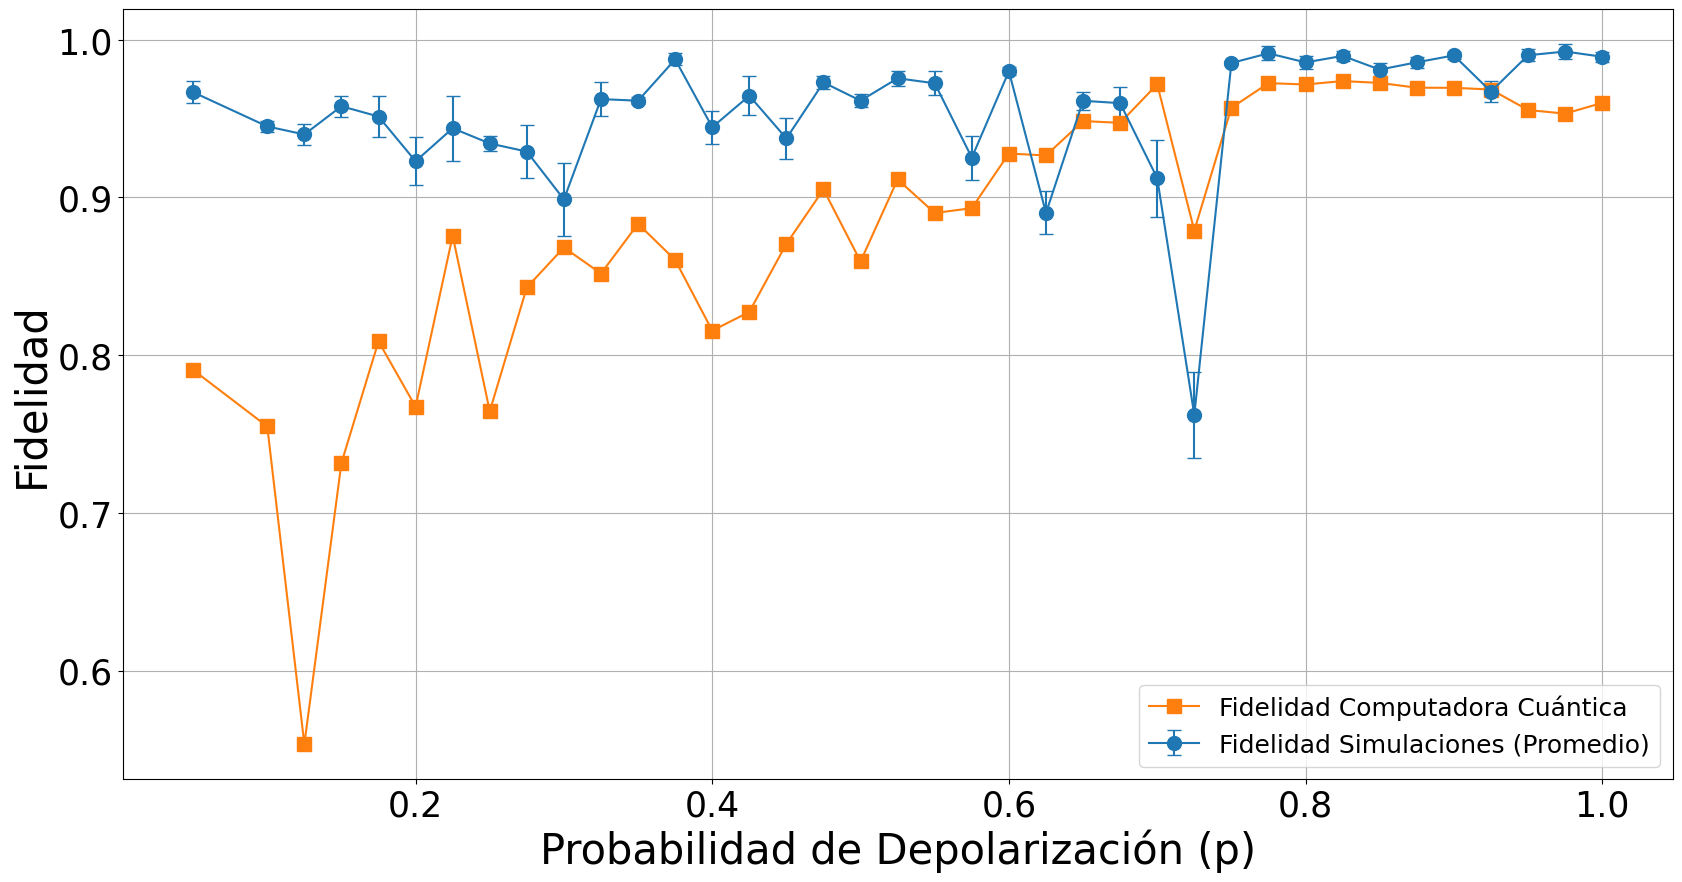
\includegraphics[width=0.7\linewidth]{imagenes/comparacion fidelidad.png}
    \caption{Comparación de fidelidades de proceso luego de ejecutar el ansatz
optimizado. En azul se encuentra la fidelidad de la matriz de Choi reconstruida
en el simulador cuántico \texttt{AerSimualtor()}. Por otro lado en azul,
corresponde a la ejecución en la computadora cuántica \texttt{ibm-kyoto}.
\textbf{Fuente}: elaboración propia. }
    \label{fig:comparacion_fidelidad}
    \end{figure}
    

\begin{table}[htbp]
\centering 
\resizebox{\textwidth}{!}{
\begin{tabular}{|l|c|c|c|c|c|c|c|}
\hline
\textbf{Backend} & \textbf{Mediana} & \textbf{Mínimo} & \textbf{Máximo} & \textbf{p(max)} & \textbf{p(min)} & \textbf{Desv. Estándar} \\ \hline
Aer Simulator & 0.9618  & 0.7620  & 0.9925 & 0.975 & 0.725 & 0.0418 \\ \hline
ibm-kyoto     & 0.8916 & 0.5533 & 0.9738 & 0.825 & 0.125 & 0.0899  \\ \hline
\end{tabular}
}
\caption{Comparación de fidelidad de proceso entre las matrices de Choi
reconstruidas del ansatz optimizado. Los resultados de la computadora cuántica
fueron tomados en \texttt{ibm-kyoto}, mientras que en el simulador fueron en
\texttt{AerSimualtor()} de qiskit. \textbf{Fuente:} elaboración propia.}
\label{tab:comparacion_fidelidades}
\end{table}

Como parte de la evaluación de completa positividad (CP)  de las matrices
reconstruidas, es importante analizar los autovalores de la matriz de Choi
correspondiente al depolarizing channel. Sabemos que su matriz de Choi esta
dada por la ecuación \ref{ec:Choi_depolarizing} \felnote{Aquí todavía no
aparece porque la declararemos en el capítulo 1}. Por lo tanto, sus autovalores
se calculan resolviendo:

\begin{equation}
\det(\Lambda_\mathcal{E} - \lambda I) = 0,
\end{equation}
donde $\Lambda_\mathcal{E}$ es la matriz de Choi e $I$ es la matriz identidad
de dimensiones $4 \times 4$. Para resolver esta ecuación, restamos $\lambda$ de
los elementos diagonales de $\Lambda_\mathcal{E}$:

\begin{equation}
\Lambda_\mathcal{E} - \lambda I = \begin{pmatrix}
1 - \frac{p}{2} - \lambda & 0 & 0 & 1 - p \\
0 & \frac{p}{2} - \lambda & 0 & 0 \\
0 & 0 & \frac{p}{2} - \lambda & 0 \\
1 - p & 0 & 0 & 1 - \frac{p}{2} - \lambda
\end{pmatrix}.
\end{equation}
Al encontrar la determinante de la matriz:
\begin{equation}
\left( \frac{p}{2} - \lambda \right)^2  \left[ \left( 1 - \frac{p}{2} - \lambda \right)^2 - (1 - p)^2 \right] = 0.
\end{equation}
Esto se puede factorizar como:
\begin{equation}
\left( \frac{p}{2} - \lambda \right)^2 \left( \lambda - \frac{p}{2} \right) \left( \lambda - \left( 2 - \frac{3p}{2} \right) \right) = 0.
\end{equation}
Por lo tanto, los autovalores de $\Lambda_{\mathcal{E}}$ son:
\begin{align}
\lambda_1 &=\lambda_2=\lambda_3 = \frac{p}{2} \quad \\
\lambda_4 &= 2 - \frac{3p}{2} .
\end{align}
Comparamos los autovalores de nuestros resultados en la figura
\ref{fig:comparacion_autovalores} para cada valor de $p$. Notamos que todos los
autovalores para todos los valores de $p$ cumplen con ser mayores o iguales a
0. Por lo que las matrices de Choi reconstruidas cumplen con ser CP.  Por otro
lado, al analizar la condición de preservación de la traza (TP) notamos que
ninguna de las matrices de Choi reconstruidas en ninguno de los sistemas cumple
con preservar la traza. Esto lo verificamos trazando parcialmente las matrices
de Choi con \texttt{partial\_trace()}, cuyo resultado no coincide con la matriz
identidad $I$. 
\begin{figure}[h!] 
    \centering 
    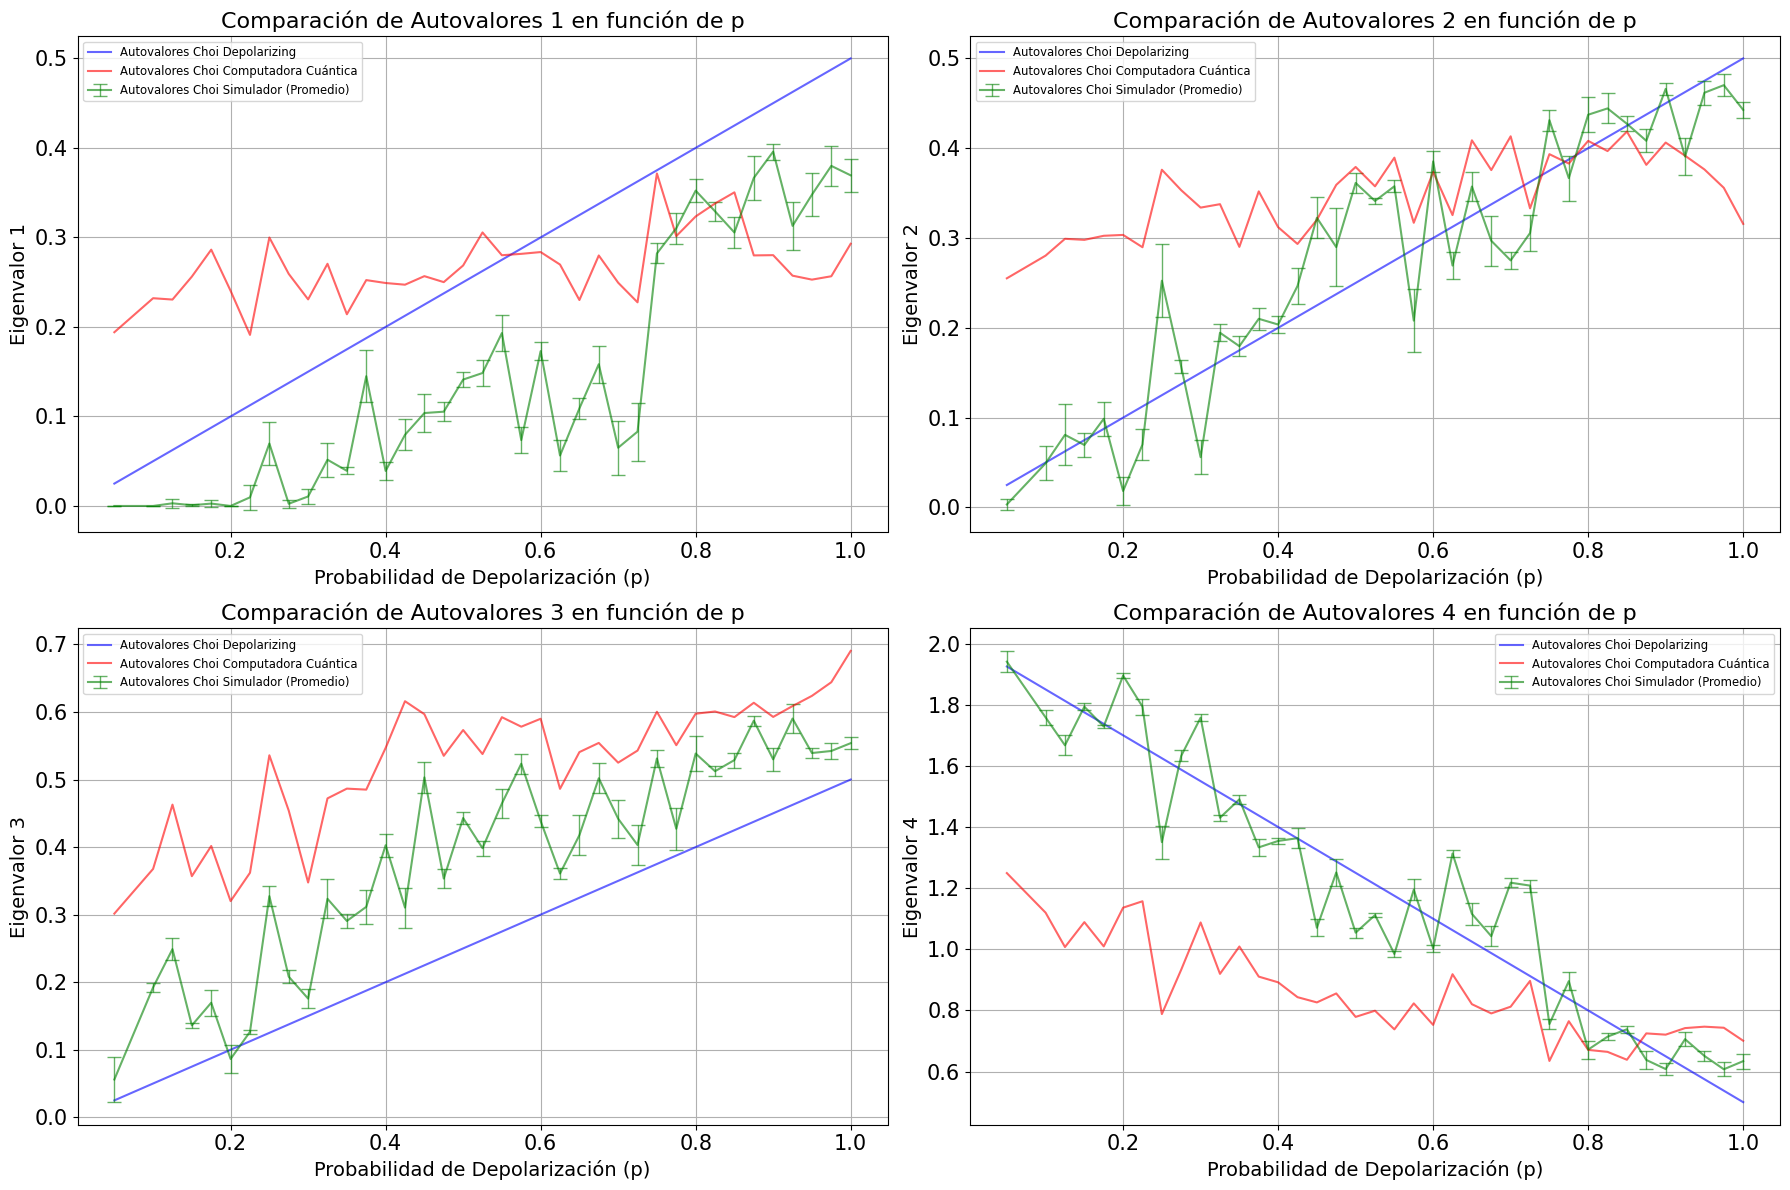
\includegraphics[width=0.90 \linewidth]{imagenes/eigenvalores_comparacion.png}
    \caption{Comparación de autovalores correspondientes a la matriz de Choi reconstruidas. En azul se puede ver el autovalor esperado a lo largo de $p$, en verde vemos el promedio de los valores de las matrices de Choi reconstruidas  en el simulador cuántico \texttt{AerSimualtor()}. Finalmente vemos en rojo los autovalores correspondientes a las matrices de Choi reconstruidas en la computadora cuántica \texttt{ibm-kyoto}. \textbf{Fuente}: elaboración propia. }
    \label{fig:comparacion_autovalores}
\end{figure}
% }}}
\section{Discusión de Resultados} % {{{
En esta sección discutiremos sobre las diferencias encontradas entre las
fidelidades y autovalores calculados en el simulador y la computadora cuántica.
Vemos que estas diferencias se deben en gran parte a los errores inherentes al
hardware cuántico real, como la decoherencia, errores en las compuertas
cuánticas y limitaciones en la precisión de las mediciones. 

La figura \ref{fig:comparacion_fidelidad} así como la tabla
\ref{tab:comparacion_fidelidades} muestran que el simulador cuántico produce
resultados con fidelidades consistentemente cercanas a 1 a lo largo de todo el
rango de $p$. En contraste, la computadora cuántica presenta una mayor
variabilidad en sus resultados. Para analizar esta diferencia, realizamos una
regresión lineal de la fidelidad en función de $p$ tanto para la computadora
cuántica como para el simulador, como se muestra en la figura
\ref{fig:comparacion_regresiones}.

\begin{figure}[h!]
    \centering
    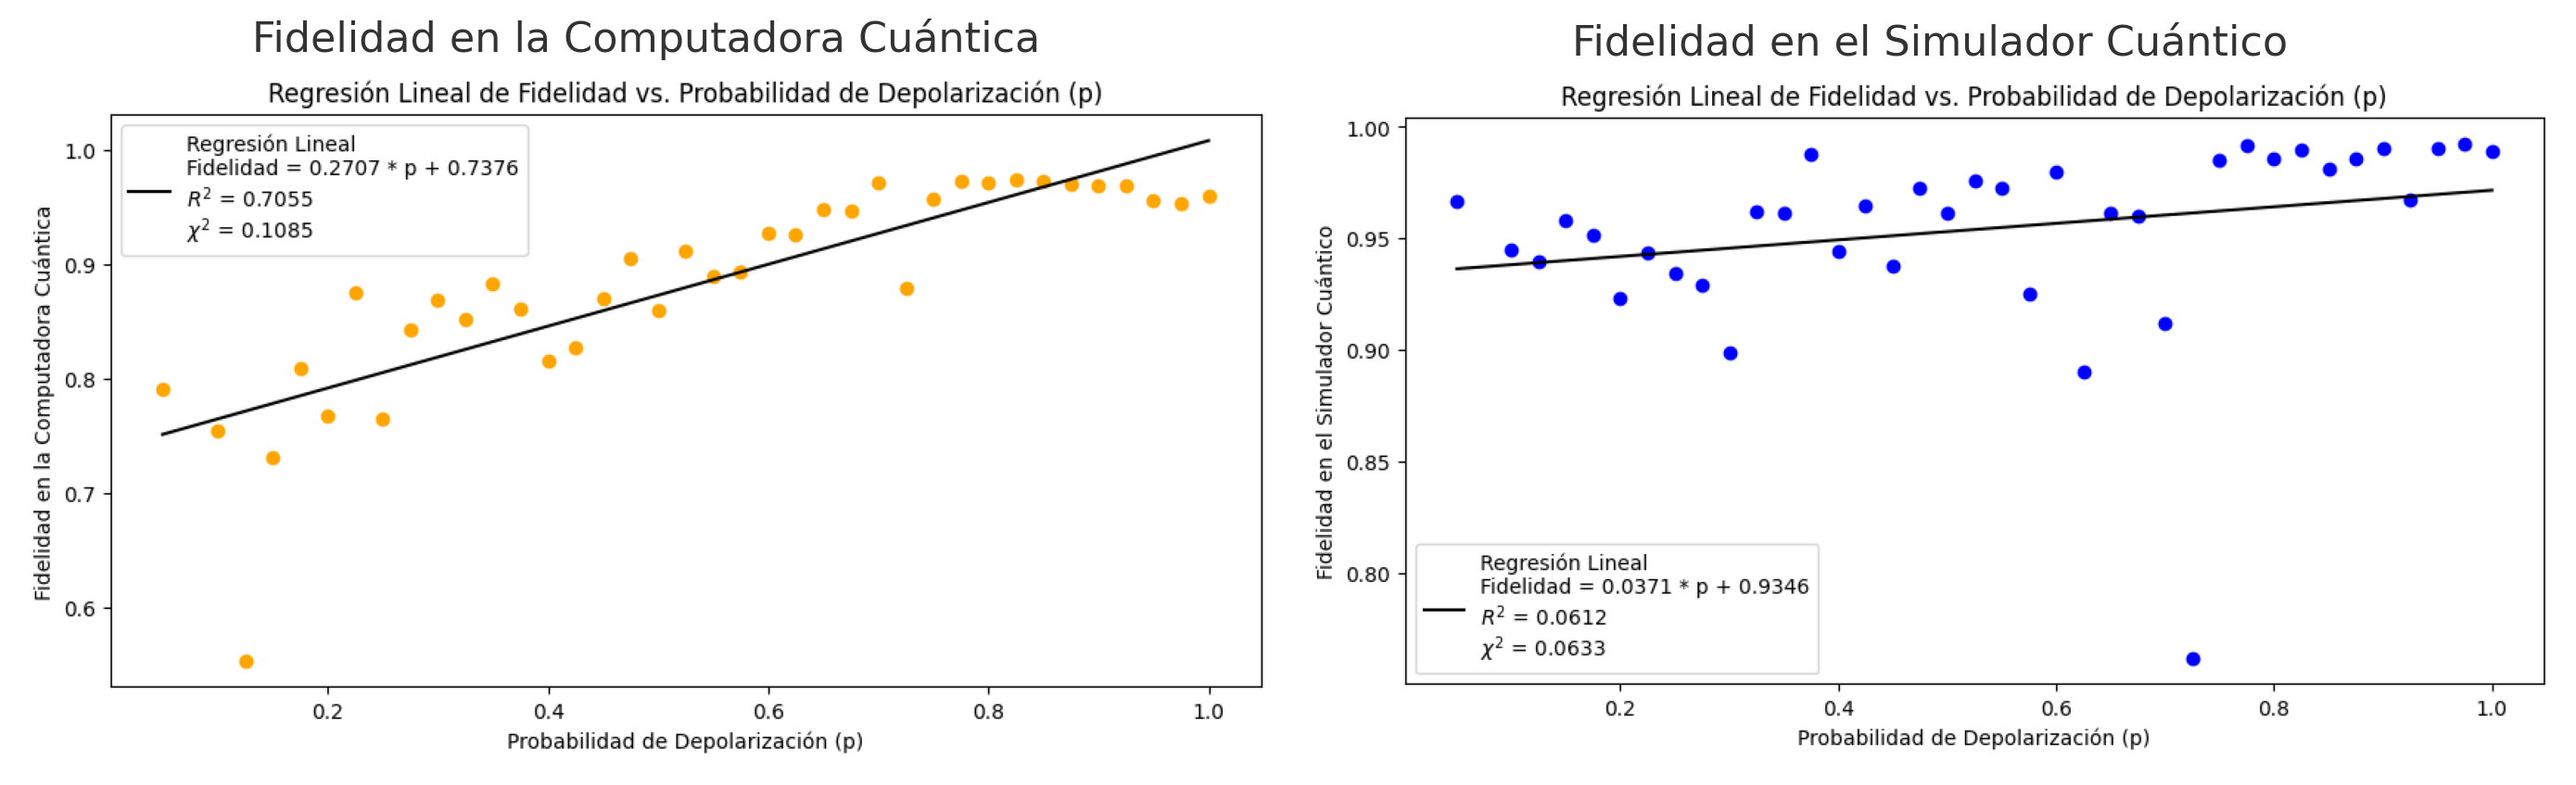
\includegraphics[width=0.95\linewidth]{imagenes/Comparacion_regresiones.png}
    \caption{Comparación de regresiones lineales entre los resultados de la fidelidad de proceso entre la matriz de Choi esperada , la computadora cuántica \texttt{ibm\_kyoto} y el simualdor cuántico \texttt{AerSimualtor()} respectivamente. \textbf{Fuente:} elaboración propia.}
    \label{fig:comparacion_regresiones}
\end{figure}

En el caso de la computadora cuántica, la ecuación de la regresión lineal es:

\begin{equation}
    F_{proc\_qc}(p) = 0.2707 \cdot p + 0.7376,
\end{equation}

con un coeficiente de determinación $R^2 = 0.7055$ y un valor de Chi-cuadrado de $\chi^2 = 0.1085$. Esta ecuación indica que la fidelidad en la computadora cuántica aumenta proporcionalmente a $p$. Este comportamiento podría deberse a que, al aumentar la probabilidad de depolarización, también se incrementa la decoherencia en el sistema. En consecuencia, la computadora cuántica \texttt{ibm\_kyoto} parece ofrecer mejores resultados de fidelidad cuando hay una mayor interacción con el entorno.

Por otro lado, observamos que el simulador \texttt{AerSimulator()} tiene una ecuación de la recta:
\begin{equation}
    F_{proc\_sim}(p) = 0.0371 \cdot p + 0.9346,
\end{equation}
con un coeficiente de determinación $R^2 = 0.0612$ y un valor de Chi-cuadrado de $\chi^2 = 0.0633$. El bajo valor de $R^2$ en el simulador sugiere que, a diferencia de la computadora cuántica, la fidelidad en el simulador no parece depender significativamente de $p$. Además, la pendiente de la recta es pequeña, lo que indica que la fidelidad en el simulador es prácticamente constante a lo largo del rango de $p$.

Analizamos la variabilidad de fidelidad en ambos casos, como se muestra en la figura \ref{fig:comparacion_desviaciones}. En el simulador cuántico, no se observa una tendencia clara en la desviación estándar de la fidelidad a lo largo de $p$, excepto en el intervalo $0.6 \le p \leq 0.75$, que parece ser una anomalía en los datos. Por otro lado, la computadora cuántica muestra una reducción en la desviación estándar de la fidelidad a medida que aumenta $p$, lo que confirma nuestra suposición basada en la regresión lineal. Finalmente, en ambos casos, observamos que para valores de $p>0.75$, la desviación estándar disminuye significativamente.


\begin{figure}[h!]
    \centering
    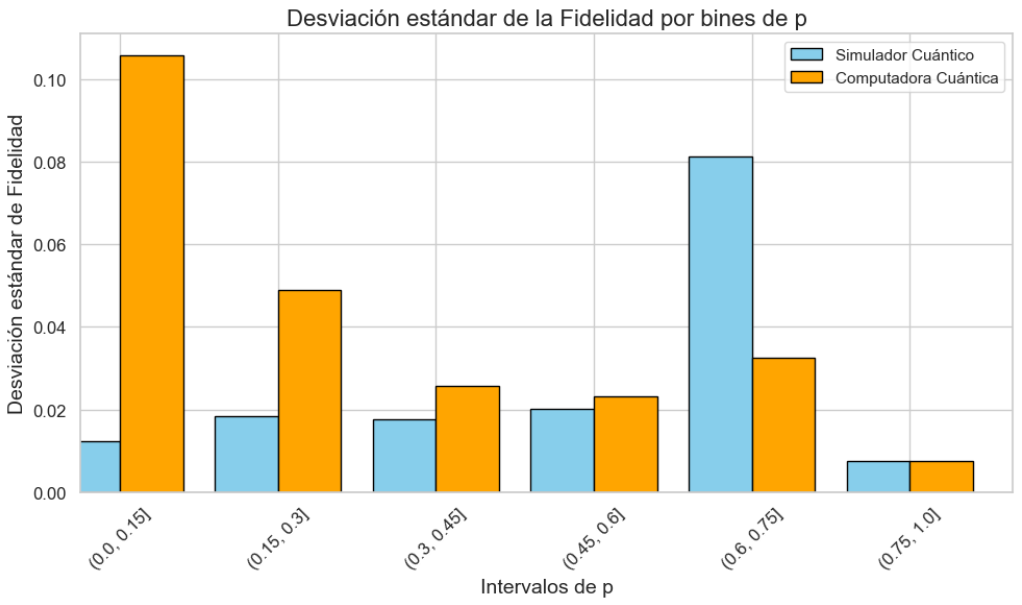
\includegraphics[width=0.95\linewidth]{imagenes/Comparacion_desviaciones.png}
    \caption{Comparación de desviación estándar entre los resultados de la fidelidad de proceso entre la matriz de Choi esperada , la computadora cuántica \texttt{ibm\_kyoto} (color naranja) y el simualdor cuántico (color azul) \texttt{AerSimualtor()}. La desviación estándar se calcula sobre los valores de fidelidad en el intervalo de $p$. \textbf{Fuente:} elaboración propia.}
    \label{fig:comparacion_desviaciones}
\end{figure}


Al analizar los cuatro autovalores presentados en la figura
\ref{fig:comparacion_autovalores}, notamos que tanto en el simulador como en la
computadora cuántica, los autovalores $\lambda_1,\lambda_2,\lambda_3$ no son
iguales entre sí. Además, en todos los casos, la computadora cuántica se desvía
más de los resultados esperados en comparación con el simulador.
Específicamente, observamos que la computadora cuántica comienza con valores
más altos para $\lambda_1,\lambda_2,\lambda_3$, y también con valores más bajos
para $\lambda_4$ en comparación con el simulador.  Estos primeros tres
autovalores están relacionados con la probabilidad de que el canal mantenga el
estado cuántico original, mientras que el cuarto autovalor corresponde a la
probabilidad de que el estado cuántico se vuelva completamente mixto. Por lo
tanto, estas observaciones sugieren que la computadora cuántica introduce más
ruido desde etapas tempranas, que se refleja en una tendencia menos pronunciada
en comparación con el simulador. Esta interpretación es coherente con los
resultados obtenidos en la regresión lineal, donde el intercepto de la
fidelidad en la computadora cuántica ($0.7376$) es menor que en el simulador,
que muestra fidelidades iniciales más altas y con menor variabilidad
($0.9346$).

En la figura \ref{fig:comparacion_choi}, observamos que las matrices de Choi
generadas por la computadora cuántica presentan mayor coherencia en las
entradas no diagonales. Esto también nos muestra que la computadora cuántica
introduce ruido desde un inicio. Notemos que al incrementar $p$, introducimos
más ruido a la interacción, que hace que nuestra fidelidad mejore con la
computadora cuántica. Por otro lado , las matrices obtenidas del simulador son
más consistentes con los vlores teóricos, con valores casi nulos en las
posiciones no diagonales, reflejando mayor fidelidad en la simulación del canal
a lo largo de $p$.

\begin{figure}[h!]
    \centering
    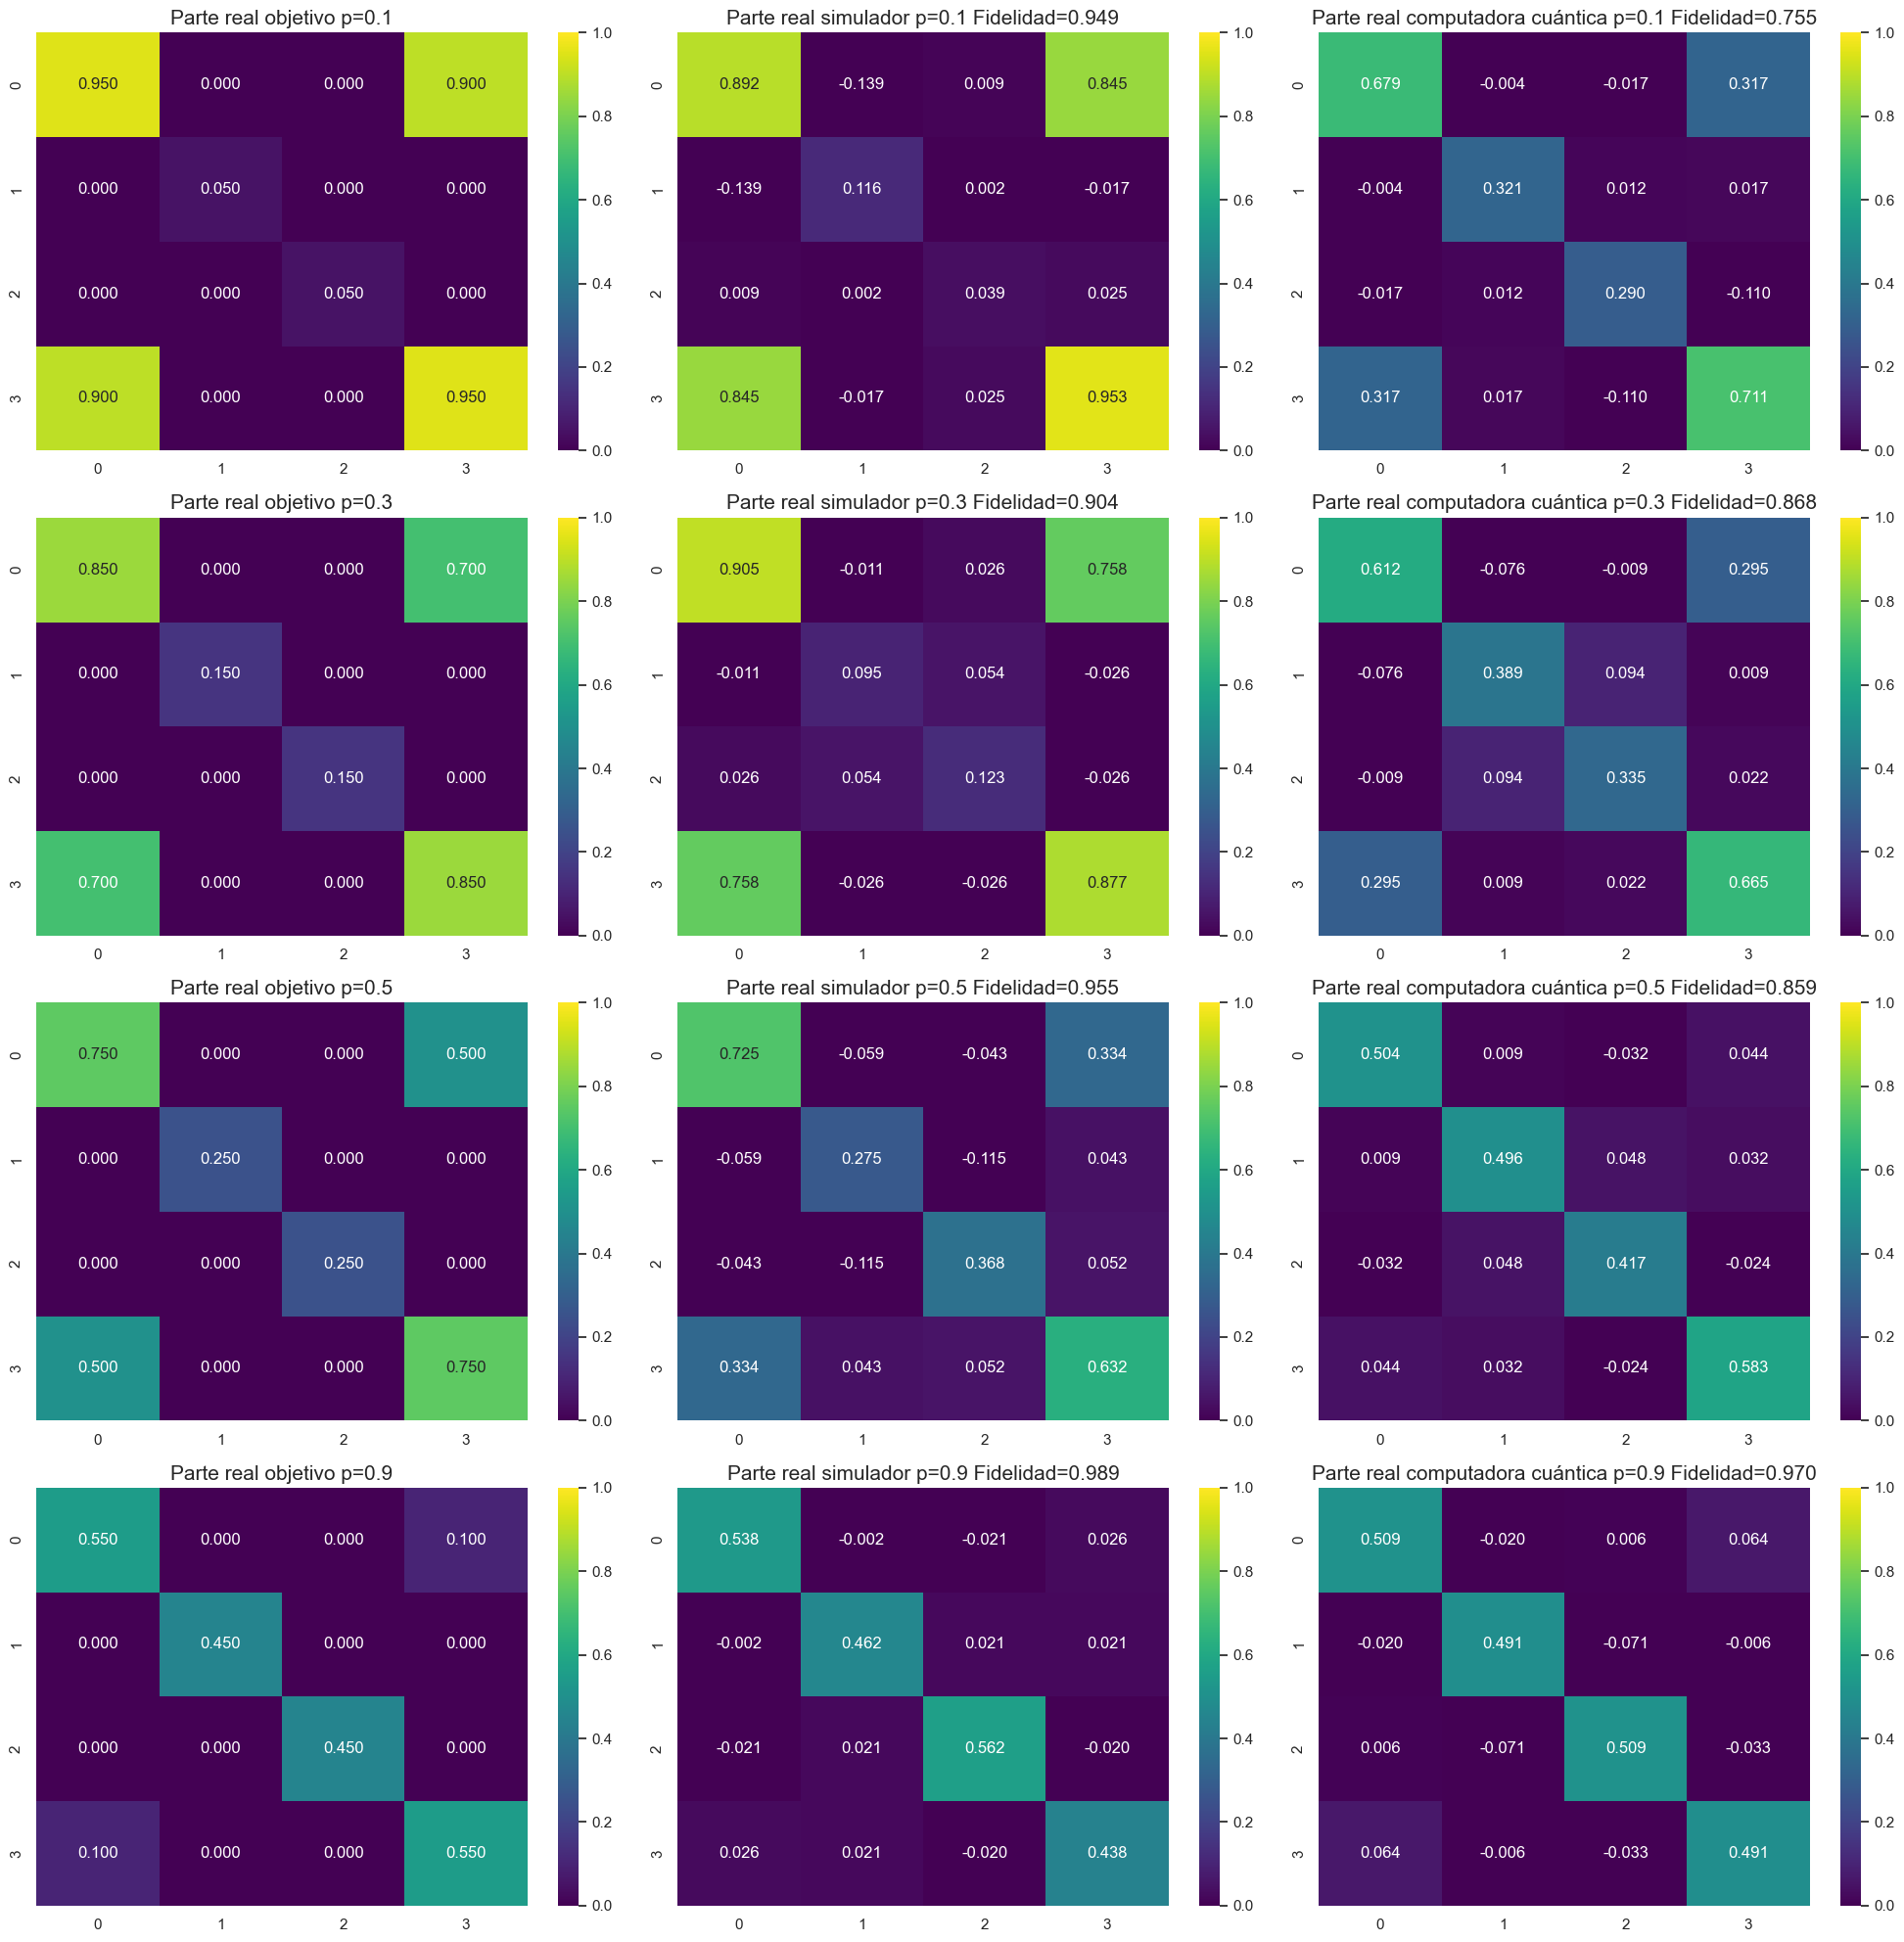
\includegraphics[width=0.95\linewidth]{imagenes/comparacion_choi.png}
    \caption{Comparación de matrices de Choi objetivo, y matrices de Choi reconstruidas en el simulador cuántico \texttt{AerSimulator()} como en la computadora cuántica \texttt{ibm\_kyoto} respectivamente. \textbf{Fuente:} elaboración propia.}
    \label{fig:comparacion_choi}
\end{figure}

% }}}
% }}}
\chapter{CONCLUSIONES} % {{{
\section{Conclusiones}
\section{Trabajo a Futuro}
\subsection{Implementación de VQA para 2 qubits}
% }}}
\appendix
% Notas sueltas {{{

% En la teoría cuántica, un sistema cuántico abierto es aquel que no está aislado, sino que interactúa continuamente con su entorno. Este tipo de sistemas son fundamentales para entender muchos fenómenos cuánticos en la práctica, ya que cualquier sistema cuántico real interactúa con su entorno. A diferencia de los sistemas cuánticos cerrados, que se consideran completamente aislados y evolucionan de manera unitaria según la ecuación de Schrödinger, los sistemas cuánticos abiertos pueden sufrir pérdidas de coherencia cuántica debido a estas interacciones. En la sección 3.1 exploraremos este tipo de sistemas por medio de canales cuánticos, con énfasis en su representación con la matriz de Choi. En la sección 3.2 mencionaremos la tomografía y fidelidad de proceso cuántico, ya que son importantes para la reconstrucción de canales cuánticos en computadoras cuánticas


% % Pendiente de redactar
% Los Algoritmos Variacionales Cuánticos (VQA) representan una estrategia innovadora en el campo de la computación cuántica para resolver problemas complejos. A través de un esquema híbrido que aprovecha tanto recursos cuánticos como clásicos, los VQA buscan optimizar un conjunto de parámetros en un circuito cuántico parametrizado. Estos algoritmos son fundamentales en tareas donde la solución se codifica dentro de una función de costo o pérdida, la cual es minimizada a través del ajuste variacional de parámetros dentro del circuito. \cite{VQA}

% El circuito cuántico parametrizado, o \textit{ansatz}, es diseñado para ser versátil y adaptarse a la naturaleza del problema y las características del hardware cuántico disponible. Los ansatz más efectivos, como el Hardware Efficient Ansatz (HEA), son aquellos que equilibran la expresividad del circuito y la eficiencia en términos de recursos y operaciones cuánticas requeridas. \cite{VQA}

% El proceso de optimización en VQAs se articula en tres fases principales:
% \begin{enumerate}
%     \item \textbf{Inicialización:} Se comienza con la preparación de un estado cuántico de referencia, sobre el cual se aplicarán las operaciones del \textit{ansatz}.
%     \item \textbf{Aplicación del Ansatz:} Se utiliza el \textit{ansatz} para transformar el estado inicial en un estado final que depende de los parámetros variacionales. Este paso es crítico y requiere una cuidadosa selección y configuración de las puertas cuánticas para navegar el espacio de Hilbert eficazmente.
%     \item \textbf{Evaluación y Optimización:} Se evalúa la función de costo mediante mediciones cuánticas y se emplea un optimizador clásico para ajustar los parámetros en busca de un mínimo, completando así el bucle cuántico-clásico.
% \end{enumerate}
% \subsubsection{Ejemplo: Inicialización de estados mixtos en computadoras cuánticas}
% Faltante de redactar




% \section{Aplicación de VQA para la simulación de Canales Cuánticos}
% Faltante de Redactar





% }}}
\bibliographystyle{abbrv}
\bibliography{references}   % Bibliografía
\end{document}
